% Paper figure: actor--critic learning and closed-loop brain intervention.
% Content follows Conclusion.tex. Redrawn as vector artwork; no slide is embedded.
% Layout styles adapted from OpenTikZ system-block-diagram (CC0-1.0).
% Template node names retained: client=state, gateway=world model, svc1=critic,
% svc2=actor, db=next state, cache=neural state estimator, backend=rollout group.
% Rebuild: make figure-brain-loop
\documentclass[border=3pt]{standalone}
\usepackage[T1]{fontenc}
\usepackage{newtxtext,newtxmath}
\usepackage{tikz}
\usetikzlibrary{arrows.meta,calc,fit,backgrounds}
\definecolor{otblue}{HTML}{0072B2}
\definecolor{otorange}{HTML}{E69F00}
\definecolor{otteal}{HTML}{009E73}
\definecolor{otpurple}{HTML}{CC79A7}
\definecolor{otgray}{HTML}{5A5A5A}

% Dimensions and labels in one place; units are cm.
\def\FigureWidth{16.2}
\def\PanelTop{5.55}
\def\StateY{2.75}
\def\HeadY{4.25}
\def\ActorY{0.85}
\def\StateX{1.05}
\def\ModelX{3.70}
\def\NextX{6.15}
\def\BrainX{9.20}
\def\EstimateX{13.60}
\def\PanelBX{8.00}
\def\boxminw{1.8}
\def\boxminh{0.76}
\def\clientlabel{$s_t=(h_t,z_t)$}
\def\gatewaylabel{Brain world\\model}
\def\svconelabel{Critic $v$}
\def\svctwolabel{Actor $\pi$}
\def\dblabel{$s_{t+1}$}
\def\cachelabel{Neural state\\estimation}
\def\grouplabel{Imagined transition}
\def\TrainingTitle{(a) Actor--critic learning}
\def\InterventionTitle{(b) Closed-loop intervention}
\def\BrainLabel{Brain}
\def\PolicyLabel{Policy $\pi$}
\def\StimulationLabel{tFUS}
\def\DecoderLabel{Pain decoder}

\begin{document}
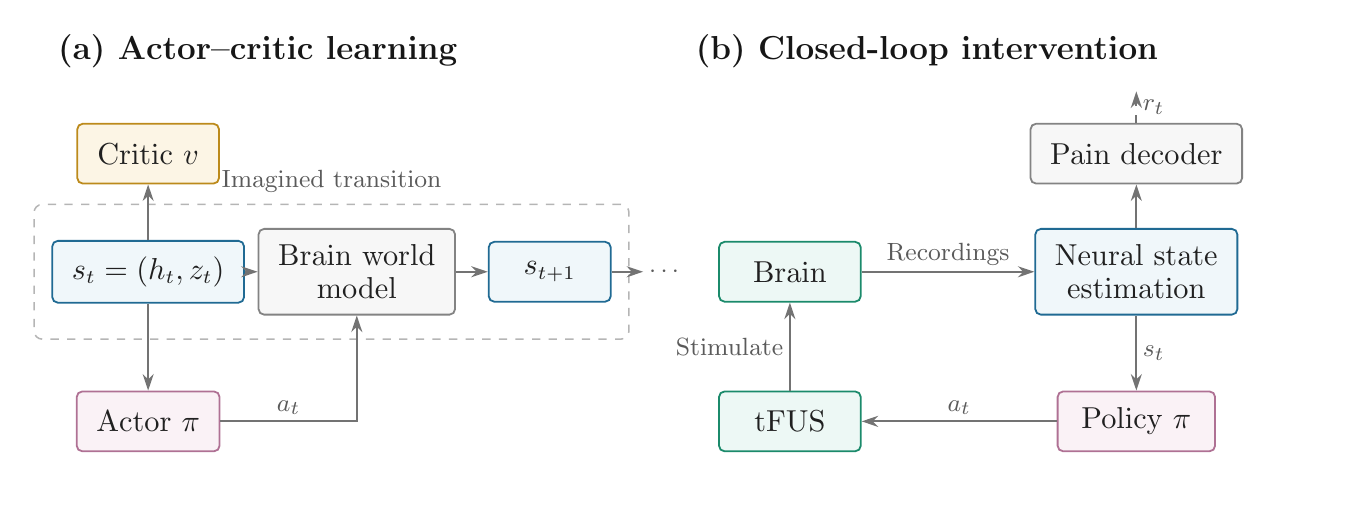
\begin{tikzpicture}[x=1cm,y=1cm,
    font=\fontsize{10.5}{12}\selectfont,
    text=otgray!35!black,
    >={Stealth[length=2.1mm,width=1.4mm]},
    comp/.style={rounded corners=2pt,line width=0.65pt,align=center,
      minimum width=\boxminw cm,minimum height=\boxminh cm,
      inner xsep=0.25cm,inner ysep=0.20cm},
    process/.style={comp,draw=otblue!65!otgray,fill=otblue!6},
    external/.style={comp,draw=otteal!70!otgray,fill=otteal!7},
    actor/.style={comp,draw=otpurple!75!otgray,fill=otpurple!10},
    critic/.style={comp,draw=otorange!70!otgray,fill=otorange!10},
    model/.style={comp,draw=otgray!75,fill=otgray!5},
    link/.style={->,draw=otgray!85,line width=0.8pt},
    group/.style={rounded corners=3pt,draw=otgray!45,dashed,
      line width=0.55pt,inner xsep=0.22cm,inner ysep=0.30cm},
    label/.style={font=\fontsize{9.5}{11}\selectfont,text=otgray,inner sep=2pt},
    title/.style={anchor=west,font=\fontsize{11.5}{13}\selectfont\bfseries,
      text=otgray!25!black,inner sep=0pt}
  ]
  \path[use as bounding box] (-0.48,0.10) rectangle (\FigureWidth,5.85);
  \node[title] at (-0.10,\PanelTop) {\TrainingTitle};
  \node[title] at (\PanelBX,\PanelTop) {\InterventionTitle};

  % (a) One learned brain state supplies both actor and critic readouts.
  \node[process] (client) at (\StateX,\StateY) {\clientlabel};
  \node[critic] (svc1) at (\StateX,\HeadY) {\svconelabel};
  \node[actor] (svc2) at (\StateX,\ActorY) {\svctwolabel};
  \node[model,minimum width=1.90cm,minimum height=1.03cm]
    (gateway) at (\ModelX,\StateY) {\gatewaylabel};
  \node[process,minimum width=1.55cm] (db) at (\NextX,\StateY) {\dblabel};
  \draw[link] (client) -- (svc1);
  \draw[link] (client) -- (svc2);
  \draw[link] (client) -- (gateway);
  \draw[link] (svc2.east) -- (\ModelX,\ActorY)
    node[midway,above,label] {$a_t$} -- (gateway.south);
  \draw[link] (gateway) -- (db);
  \draw[link] (db.east) -- ++(0.40,0);
  \node[label,anchor=west] at ([xshift=0.40cm]db.east) {$\cdots$};
  \begin{scope}[on background layer]
    \node[group,fit=(client)(gateway)(db)] (backend) {};
  \end{scope}
  \node[label,anchor=south] at ([yshift=0.06cm]backend.north) {\grouplabel};

  % (b) A deployed policy selects stimulation; new recordings close the loop.
  \node[external] (brain) at (\BrainX,\StateY) {\BrainLabel};
  \node[process,minimum width=2.35cm,minimum height=1.03cm]
    (cache) at (\EstimateX,\StateY) {\cachelabel};
  \node[actor,minimum width=2.0cm]
    (execution-policy) at (\EstimateX,\ActorY) {\PolicyLabel};
  \node[external] (stimulation) at (\BrainX,\ActorY) {\StimulationLabel};
  \node[model,minimum width=2.0cm]
    (pain-decoder) at (\EstimateX,\HeadY) {\DecoderLabel};

  \draw[link] (brain) -- (cache) node[midway,above,label] {Recordings};
  \draw[link] (cache) -- (execution-policy) node[midway,right,label] {$s_t$};
  \draw[link] (execution-policy) -- (stimulation)
    node[midway,above,label] {$a_t$};
  \draw[link] (stimulation) -- (brain)
    node[midway,left,label] {Stimulate};
  \draw[link] (cache) -- (pain-decoder);
  \draw[link,dashed] (pain-decoder.north) -- ++(0,0.40) node[midway,right,label] {$r_t$};
\end{tikzpicture}
\end{document}
